\begin{minipage}[t]{0.4\textwidth}
\parindent=0.6cm
\begin{center}
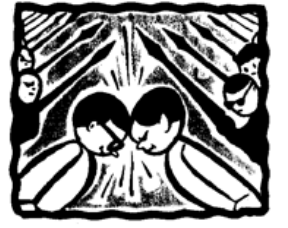
\includegraphics[]{1pic} 
\end{center}
\begin{center}
   \paragraph{Бой} 
\end{center}
\parКогда кончается время на подготовку, команды собираются вместе в зале и начинается бой, который состоит из туров (по каждой задаче). прежде всего эюри с помощью легких дополнительных вопросов, конкурса капитанов или жерьебьевкой присваивает командам номера $A, B, C$ (в дальнейшем роли команд меняются в соответствии с заранее составленным расписанием, если ни одна из команд не отказывается от вызова). \\ \indentПосле этого жюри предоставляет право команде $A$ вызвать команду $B$ на любую задачу, которая решена командой $A$ и еще не рассказывалась. Если команда $A$ не имеет таких задач, то она может отказаться от вызова, но при всём этом она лишится права\\
\end{minipage}%
\hfill
\hfill
\begin{minipage}[t]{0.4\textwidth}
\parindent=0.6cm
\begin{center}
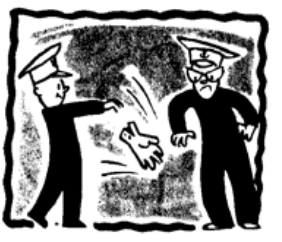
\includegraphics[]{2pic} \\
\end{center}
выступать до конца боя. Поэтому иногда команда сознательно делает вызов на нерешенную задачу. Если это в дальнейшем обнаруживается, то классифицируется как "некорректный вызов" и соответствующим образом карается.\\
\indentДалее возможны 9 вариантов, собранные в таблицу 1. \\ \indent
Команда $B$ может принять вызов, либо может отказаться рассказывать решение. В случае отказа проверяется корректность вызова: решение обязана рассказать команда $A$. Если команда знает решение, но не может четко рассказать его или подозревает, что в решении есть ошибки, часто бывает выгоднее отказаться отвечать. Одна из команд $A$ или $B$ назначает отвечающего решение, другая--оппонента. Команда $C$ сразу же назначает
\end{minipage}

\begin{center}
\paragraph{9 выриантов распределения ролей 3 команд в туре } \\
\end{center}


\begin{tabular}{|c|c|c|c|c|c|c|c|c|} 
\toprule
\hline
\setrow{\bfseries}A &B  &A   &C   &B  &отв. &опп. &рец. &штраф   \\ 
\hline
\midrule
  вызов B   &принят  &--  &--  &-- &B &A &$C$ &--  \\
  \cline{2-9}
  вызов B  &отказ  &принят  &--  &-- &A(?) &B &C &? \\
  \cline{3-9}
  вызов B  &отказ  &\multirow{3}*{отказ (некорр.вызов)}  &принят  &-- &C &B &A &A \\ 
  \cline{4-9}
  вызов B  &отказ &--  &отказ  &-- &-- &-- &-- &A \\
  \hline
  отказ &вызов C  &-- &принят  &-- &C &B &A &-- \\
  \cline{4-9}
  отказ &вызов C  &-- &отказ  &принят &B(?) &C &A &? \\
  \cline{5-9}
  отказ &вызов C  &-- &отказ  &отказ(некорр.вызов) &-- &-- &-- &B \\
  \cline{2-9}
  отказ &отказ &-- &принят  &-- &C &B &A &-- \\
  \cline{4-9}
  отказ &отказ &-- &отказ  &-- &-- &-- &-- &-- \\
\hline
\bottomrule
\end{tabular}
